
\usetikzlibrary{decorations.text}
\usetikzlibrary{calc}
\usetikzlibrary{fit}
\usetikzlibrary{shapes}
\usetikzlibrary{arrows,positioning} 

%\begin{document}
\begin{figure}[h]
\begin{center}
\scalebox{1}{
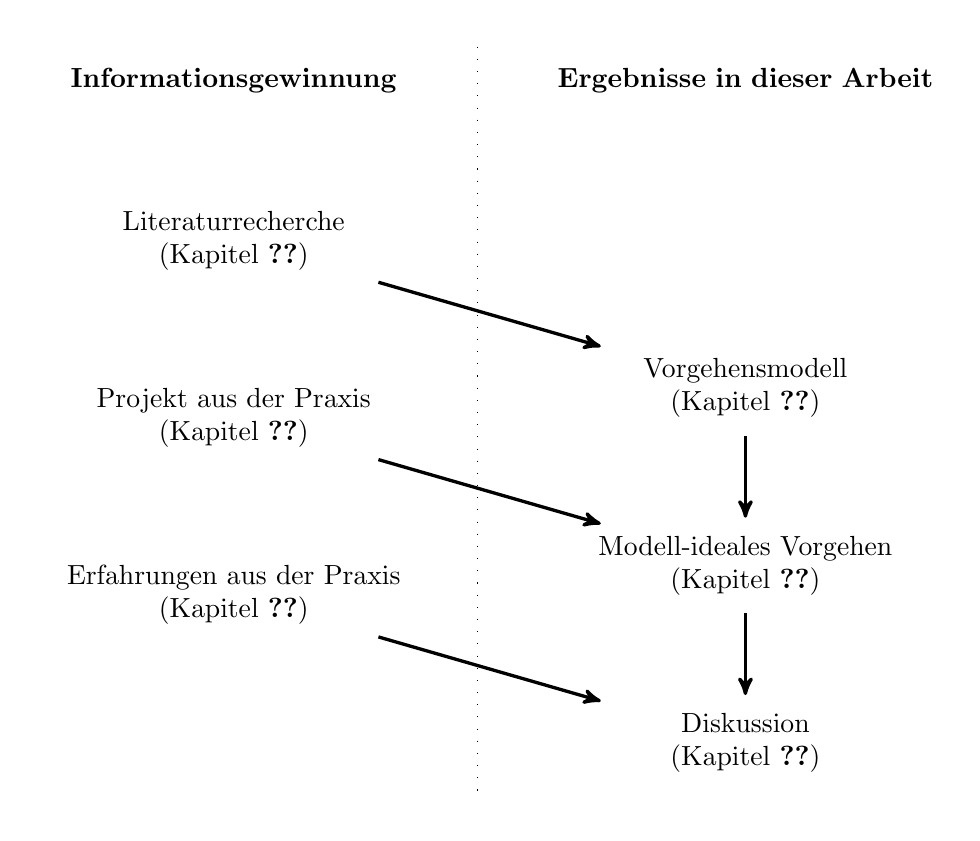
\begin{tikzpicture}[
	node distance=1.25cm,
	auto,
	pile/.style={
		very thick,
		->,
		>=stealth',
		shorten <=3pt,
		shorten >=3pt
	},
	knoten/.style={
		text width=5cm,
		text centered
	}
]
\node[knoten] (INFOS)  {\textbf{Informationsgewinnung}};
\node[knoten] (ERG) [right=of INFOS] {\textbf{Ergebnisse in dieser Arbeit}};

\node[knoten] (LIT) [below=of INFOS]
{Literaturrecherche\\(Kapitel~\ref{cha:literaturuebersicht})};

\node[knoten] (INV) [below=of ERG, right=of LIT] {};


\node[knoten] (PROJ) [below=of LIT] {Projekt aus 
der Praxis\\(Kapitel~\ref{cha:replyundifms})};

\node[knoten] (VOR) [right=of PROJ, below=of INV] 
{Vorgehensmodell\\(Kapitel~\ref{cha:entwicklung_vorgehensmodell})};


\node[knoten] (IDEAL) [below=of VOR] 
{Modell-ideales Vorgehen\\(Kapitel~\ref{cha:result})};

\node[knoten] (ERF) [below=of PROJ] {Erfahrungen aus 
der Praxis\\(Kapitel~\ref{cha:praxis})};

\node[knoten] (DISK) [below=of IDEAL] 
{Diskussion\\(Kapitel~\ref{cha:diskussion})};

\node[above left = 0.15cm and 0.65cm of ERG] (o) {};
\node[below left = 0.15cm and 0.65cm of DISK] (u) {};

\draw[loosely dotted] (o) -- (u);

\draw[pile] (LIT) -> (VOR);
\draw[pile] (VOR) -> (IDEAL);
\draw[pile] (PROJ) -> (IDEAL);
\draw[pile] (IDEAL) -> (DISK);
\draw[pile] (ERF) -> (DISK);

\end{tikzpicture}
}
\caption{Einfluss der Forschungsmethoden in die Arbeit}
\label{fig:einfluss_forschungsmethoden}
\end{center}
\end{figure}
